\uuid{ofSt}
\titre{Fonction Logarithmique}
\chapitre{Fonction de plusieurs variables}
\niveau{L2}
\module{Analyse}
\sousChapitre{Dérivées partielles}
\theme{}
\auteur{Grégoire Menet}
\datecreate{2025-03-20}
\organisation{AMSCC}

\difficulte{}
\contenu{
	
	\texte{
		On considère la fonction définie par $f(x,y)=\ln(4-x^2-y^2)$.
	}
	
	\begin{enumerate}
		\item \question{Déterminer le domaine de définition de $f$ et le représenter graphiquement.}
		\indication{}
		\reponse{L'expression $f(x,y)$ existe si et seulement si $4-x^2-y^2>0$. Ainsi le domaine de définition de $f$ est :
			$\mathcal{D}_f=\left\{\left.(x,y)\in \R^2\right|\ x^2+y^2<4\right\}$. Il s'agit du disque ouvert de rayon 2 et de centre $(0,0)$.}
		\item \question{Déterminer la courbe de niveau $k=0$ de $f$ (donner son équation et sa nature géométrique).}
		\indication{}
		\reponse{On regarde $f(x,y)=0$. Ce qui donne $4-x^2-y^2=1$, c'est à dire $x^2+y^2=3$. Il s'agit du cercle de centre $(0,0)$ et de rayon $\sqrt{3}$.}
		\item \question{Calculer les dérivées partielles de $f$ en un point $(x,y)$ dans le domaine de définition de $f$.}
		\indication{}
		\reponse{On a :
			$$\frac{\partial f}{\partial x}(x,y)=\frac{-2x}{4-x^2-y^2}\ \ \text{et}\ \ \frac{\partial f}{\partial x}(x,y)=\frac{-2y}{4-x^2-y^2}.$$}
		\item
\question{ 		Parmi les figures suivantes laquelle correspond au graphe de $f$ ? Justifier votre réponse. 
\begin{center}
	\begin{minipage}[t]{0.45\textwidth}
		\centering
		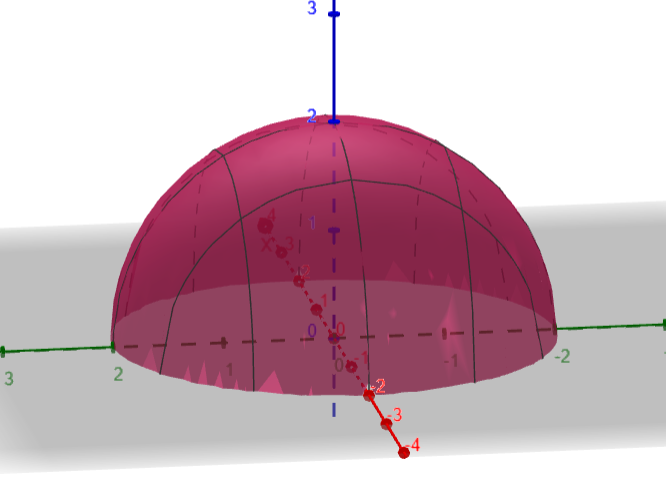
\includegraphics[width=\textwidth]{ofSt-2}
		
		Figure 1
	\end{minipage}
	\hfill
	\begin{minipage}[t]{0.45\textwidth}
		\centering
		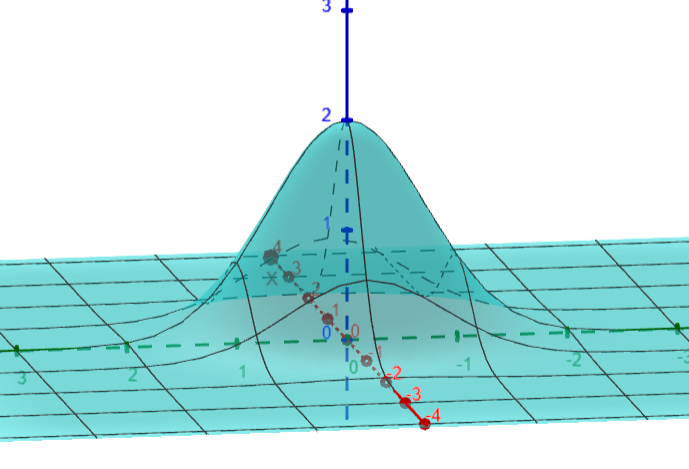
\includegraphics[width=\textwidth]{ofSt-3}
		
		Figure 2
	\end{minipage}
	
	\vspace{1em}
	
	\begin{minipage}[t]{0.45\textwidth}
		\centering
		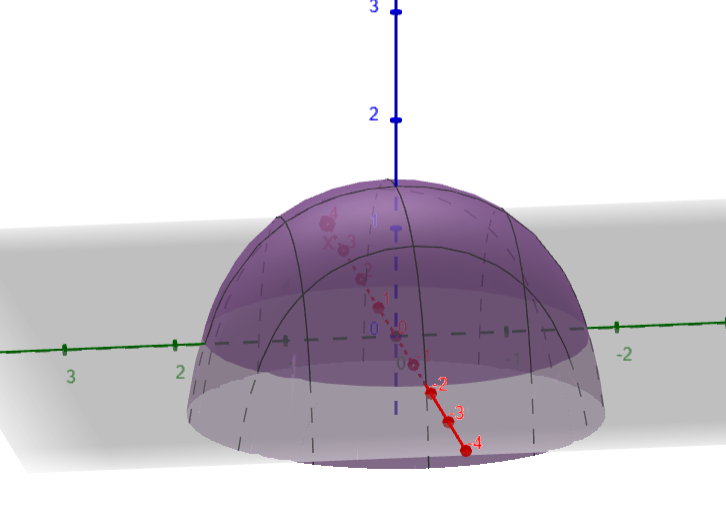
\includegraphics[width=\textwidth]{ofSt-1}
		
		Figure 3
	\end{minipage}
	\hfill
	\begin{minipage}[t]{0.45\textwidth}
		\centering
		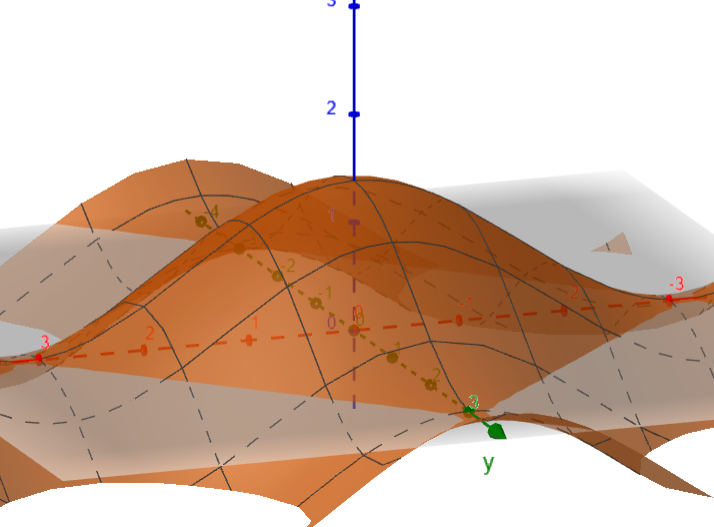
\includegraphics[width=\textwidth]{ofSt-4}
		
		Figure 4
	\end{minipage}
\end{center} }
	\reponse{ La figure 3 est correcte : on peut regarde $f(0,0) = \ln(4)$ et constater que la fonction prend des valeurs positives et négatives sur son ensemble de définition. }
	\end{enumerate}
	
}
